\documentclass[11pt, addpoints, answers]{exam}

\usepackage{amsmath, amssymb, amsthm, euler}
\usepackage{xcolor}
\usepackage{graphicx}
\usepackage{graphics}
\usepackage{tikz}
\usepackage{tikz-qtree}
\usetikzlibrary{graphs}
\tikzset{every tree node/.style={minimum width=2em,draw,circle},
    blank/.style={draw=none},
    edge from parent/.style=
    {draw,edge from parent path={(\tikzparentnode) -- (\tikzchildnode)}},
    level distance=1.2cm}
\usepackage{listings}   
\usepackage{caption}
\usepackage{algorithm}
\usepackage{algorithmicx}
\usepackage{algpseudocode}
\usepackage{underscore}
% \usepackage[top=2cm, bottom=2cm, left=2cm, right=2cm]{geometry}  
\makeatletter
\newcommand\dlmu[2][2.5cm]{\hskip1pt\underline{\hb@xt@ #1{\hss#2\hss}}\hskip3pt}
\makeatother

% For inserting code snippets.
\usepackage{listings}
\lstset{
    columns = fixed,
    basewidth = {0.5em},
    breaklines = true,
    backgroundcolor = \color{white},
    keywordstyle = \color[RGB]{40, 40, 255},
    numberstyle = \footnotesize\color{darkgray},
    commentstyle = \ttfamily\color{violet},
    basicstyle = \ttfamily,
    stringstyle = \ttfamily\color[RGB]{128, 0, 0},
    showstringspaces = false,
    language = {[11]C++},
    escapechar = \@
}
\lstnewenvironment{cpp}[1][]{\lstset{language = {[11]C++}, #1}}{}

\usepackage{tikz}

% headers, footers, titles
\newcommand{\CourseName}{CS101 Algorithms and Data Structures}
\newcommand{\HomeworkNO}{Homework 5}
\newcommand{\DueDate}{Due date: 23:59, October 23th, 2022}

\pagestyle{headandfoot}
\runningheadrule
\runningheader{\CourseName}{\HomeworkNO}{\DueDate}
\runningfooter{}{\thepage}{}

\title{
	\CourseName\\
	Fall 2022\\
	\HomeworkNO
}
\author{}
\date{\DueDate}

% formats of questions, choices, points, etc.
\qformat{\bf\thequestion. (\totalpoints\ points) \thequestiontitle\hfill}
\pointname{'}
\CorrectChoiceEmphasis{\bf\color{blue}}

% We frequently use this font.
\newcommand{\ttt}{\texttt}

\begin{document}

\maketitle

\begin{enumerate}
	\item Please write your solutions in English.
	\item Submit your solutions to gradescope.com.
	\item Set your FULL name to your Chinese name and your STUDENT ID correctly in Account Settings.
	\item If you want to submit a handwritten version, scan it clearly. \ttt{CamScanner} is recommended.
	\item When submitting, match your solutions to the problems correctly.
	\item No late submission will be accepted.
	\item Violations to any of the above may result in zero points.
\end{enumerate}

\begin{questions}

\titledquestion{Multiple Choices}

Each question has \textbf{one or more} correct answer(s). Select all the correct answer(s). For each question, you will get 0 points if you select one or more wrong answers, but you will get 1 point if you select a non-empty subset of the correct answers.

Write your answers in the following table.

%%%%%%%%%%%%%%%%%%%%%%%%%%%%%%%%%%%%%%%%%%%%%%%%%%%%%%%%%%%%%%%%%%%%%%%%%%%
% Note: The `LaTeX' way to answer a multiple-choices question is to replace `\choice'
% with `\CorrectChoice', as what you did in the previous questions. However, there are 
% still many students who would like to handwrite their homework. To make TA's work 
% easier, you have to fill your selected choices in the table below, no matter whether 
% you use LaTeX or not.
%%%%%%%%%%%%%%%%%%%%%%%%%%%%%%%%%%%%%%%%%%%%%%%%%%%%%%%%%%%%%%%%%%%%%%%%%%%

\begin{table}[htbp]
	\centering
	\begin{tabular}{|p{2cm}|p{2cm}|p{2cm}|p{6cm}|}
		\hline
		(a) & (b) & (c) \\
		\hline
		%%%%%%%%%%%%%%%%%%%%%%%%%%%%%%%%%%%%%%%%%%%%%%%%%%%%%%%%%%
		% YOUR ANSWER HERE.
		  BD  &  AC   &  C   \\
		%%%%%%%%%%%%%%%%%%%%%%%%%%%%%%%%%%%%%%%%%%%%%%%%%%%%%%%%%%
		\hline
	\end{tabular}
\end{table}

\begin{parts}
	\part[2] A problem in $\NP$ is $\NPC$ if:
	\begin{choices}
		\choice It can be reduced to another $\NPC$ problem in polynomial time.
		\CorrectChoice There exists a $\NPC$ problem which can be reduced to it in polynomial time.
		\choice It can be reduced to any other $\NP$ problem in polynomial time.
		\CorrectChoice Any other $\NP$ problem can be reduced to it in polynomial time.
	\end{choices}


	\part[2] Assuming that $\P\neq\NP$, which of the following problems are in $\NPC$?
	You may search the Internet for more information if you are unfamiliar with the problems.
	\begin{choices}
		\CorrectChoice \texttt{LONG-PATH}: $(G,s,t,k)$ Given an undirected graph $G$,
		determine whether there exists a simple path from \(s\) to \(t\) whose length is greater or equal to $k$.
		\choice \texttt{HALTING}: $(P,I)$ Given a compilable C++ program $P$ and the input $I$ for $P$,
		determine if $P$ runs infinitely on $I$.
		\CorrectChoice \texttt{4-SAT}: $\phi$ Given a CNF (conjunction normal form)
		where each clause is the disjunction of exactly 4 literals,
		determine whether $\phi$ is satisfiable.
		\choice \texttt{PRIME}: $n$ Given a positive integer $n$, determine whether it is a prime number.
	\end{choices}

	\part[2] For two decision problems $A$ and $B$, suppose that $A\leq_p B$.
	Which of the following statements are true?
	(Hint: there exists complexity classes that are strictly bigger than $\NP$)
	\begin{choices}
		\choice $A\in \P \implies B\in \P$
		\choice $A\in \NPC\implies B\not\in \NPC$.
		\CorrectChoice $B\in \P\implies A\in \P$.
		\choice $B\in \NPC\implies A\in \NPC$.
	\end{choices}

\end{parts}


\newpage

\titledquestion{Draw a binary tree}
\begin{parts}
    \part[3]Given the in-order and pre-order traversal of a binary tree T are IGDHBAECF and ABDGIHCEF respectively.\\
    Draw the tree T.\\
    \vspace{1cm}
    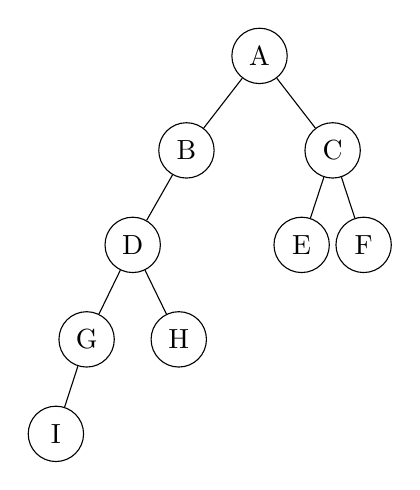
\begin{tikzpicture}
    \Tree
    [.A
        \edge[]; [.B
            \edge[]; [.D
                \edge[]; [.G
                    \edge[]; [.I ]
                    \edge[blank]; \node[blank]{};
                    ]
                \edge[]; [.H ]
                ]
            \edge[blank]; \node[blank]{};
            ]
        \edge[]; [.C
            \edge[]; [.E ]
            \edge[]; [.F ]
            ]
    ]
    \end{tikzpicture}
    \vspace{1cm}

    \part[3]Given the in-order and post-order traversal of a binary tree T are ADHGKLMRUXTW and AHDLKGUXRWTM respectively.\\
    Draw the tree T.\\
    \vspace{1cm}
    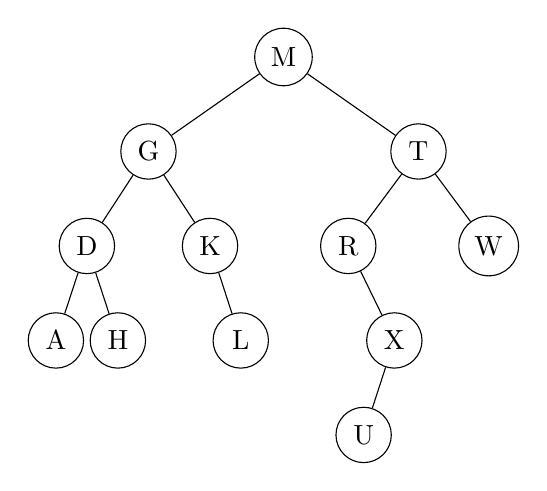
\begin{tikzpicture}
    \Tree
    [.M
        \edge[]; [.G
            \edge[]; [.D
                \edge[]; [.A ]
                \edge[]; [.H ]
                ]
            \edge[]; [.K
                \edge[blank]; \node[blank]{};
                \edge[]; [.L ]
                ]
            ]
        \edge[]; [.T
            \edge[]; [.R
                \edge[blank]; \node[blank]{};
                \edge[]; [.X
                    \edge[]; [.U ]
                    \edge[blank]; \node[blank]{};
                ]
            ]
            \edge[]; [.W ]
        ]
    ]
    \end{tikzpicture}
    \vspace{6cm}

    \part[2]Given the pre-order and post-order traversal of a binary tree T, can you decide the tree T? If yes, please describe an algorithm to construct T; if no, please provide a counterexample.
    \\
    
    \vspace{2cm}
    No.

   
    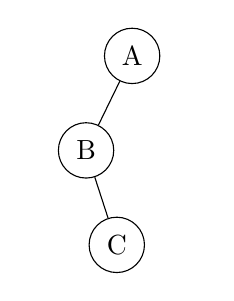
\begin{tikzpicture}
    \Tree
    [.A
        \edge[]; [.B
            \edge[blank]; \node[blank]{};
            \edge[]; [.C ]
            ]
        \edge[blank]; \node[blank]{};
    ]
    \end{tikzpicture}

    \vspace{2cm}

    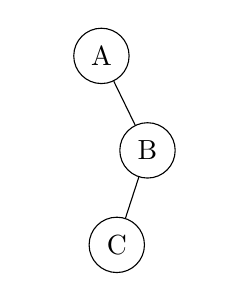
\begin{tikzpicture}
        \Tree
        [.A
            \edge[blank]; \node[blank]{};
            \edge[]; [.B
                \edge[]; [.C ]
                \edge[blank]; \node[blank]{};
                ]
        ]
    \end{tikzpicture}

    these two trees both have the \\
    pre-orfer traversal \ \ $ABC$\\
    and the post-orfer traversal \ \ $CBA$\\
    so we can not get a tree with it pre-oder and post-order traversal.
\end{parts}

\newpage

\titledquestion{Heap}
We are given the following array representing a min-heap where each letter represents a unique number. Assume the root of the min-heap is at index zero, i.e. A is the root. Note that there is no significance of the alphabetical ordering, i.e. just because B precedes C in the alphabet, we do not know if B is less than or greater than C.\\
Array: [A, B, C, D, E, F, G]\\
Six unknown operations are then executed on the min-heap. An operation is either a pop or a push.The resulting state of the min-heap is shown below\\
Array: [A, G, B, X, E, F, C]
\vspace*{0.2cm}

\begin{parts}
  \part[8]  The first and the final operations have already been filled in for you. Fill in the space below using the following options.\\
  Note: You are free to use each of the following options 0 time, once or more than once.\\
  (A) pop()\\
  (B) push(B)\\
  (C) push(C)\\
  (D) push(X)\\
  Hint: The number of elements in the heap doesn’t change after 6 operations; In the final heap, X’s position is in the left sub-heap.\\
  
  
1. pop()\\
2. \dlmu{D}\\
3. \dlmu{A}\\
4. \dlmu{A}\\
5. \dlmu{B}\\
6. push(A)
\vspace*{0.4cm}
    
  \part[4] Fill in the following comparisons with either $>$, $<$, or ? if unknown. We recommend considering which elements were compared to reach the final array.\\
  1. X\dlmu[0.5cm]{>}B\\
  2. X\dlmu[0.5cm]{>}C\\
  3. G\dlmu[0.5cm]{?}F\\
  4. G\dlmu[0.5cm]{>}D\\
\end{parts}


\newpage

\titledquestion{Heap Sort}
\begin{parts}
\part[10] You are given such a max heap like this:
\end{parts}

\begin{minipage}{1\textwidth}
\centering
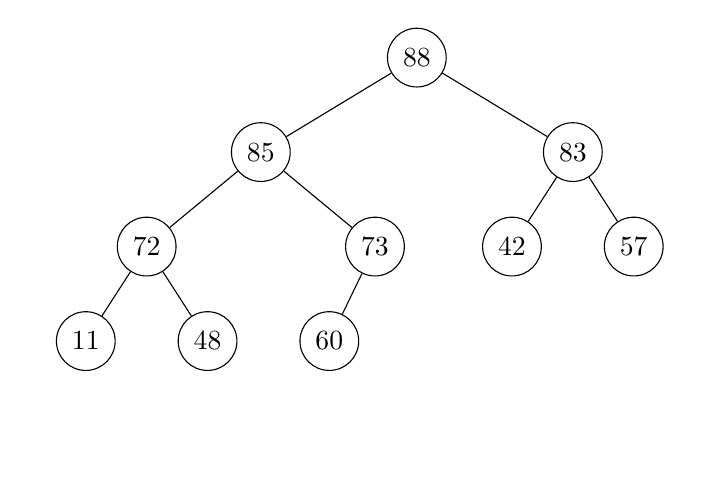
\begin{tikzpicture}
\Tree
[.88
    [.85
        \edge[]; [.72
            \edge[]; [.11
                \edge[blank]; \node[blank]{};
                \edge[blank]; \node[blank]{};
            ]
            \edge[]; [. 48
                \edge[blank]; \node[blank]{};
                \edge[blank]; \node[blank]{};
            ]
        ]
        \edge[]; [.73
            \edge[]; [.60
                \edge[blank]; \node[blank]{};
                \edge[blank]; \node[blank]{};
            ]
            \edge[blank]; \node[blank]{};
        ]
    ]
    [.83
    % \edge[blank]; \node[blank]{};
        \edge[]; [.42
            \edge[blank]; \node[blank]{};
            \edge[blank]; \node[blank]{};
        ]
        \edge[]; [.57
            \edge[blank]; \node[blank]{};
            \edge[blank]; \node[blank]{};
        ]
    ]
]
\end{tikzpicture}
\end{minipage}%

Then you need to use array method to show each step of heap sort in increasing order. Fill in the value in the table below. Notice that the value we have put is the step of each value sorted successfully. For each step, you should always make you heap satisfies the requirement of max heap property.


\begin{table}[!hbtp]
\centering
\resizebox{\textwidth}{!}{%
    \begin{tabular}{|c|c|c|c|c|c|c|c|c|c|c|c|}
        \hline
        index & 1 & 2 & 3 & 4 & 5 & 6 & 7 & 8 & 9 & 10 \\ \hline
        value & $88 $ & $85 $ &$83 $  &$72 $  & $73 $ &$42 $  &$57 $  & $11 $ &$48 $  &$60 $  \\ \hline
    \end{tabular}%
}
\caption{The original array to represent max heap.}
\label{}
\end{table}
\begin{table}[!hbtp]
\centering
\resizebox{\textwidth}{!}{%
    \begin{tabular}{|c|c|c|c|c|c|c|c|c|c|c|c|}
        \hline
        index & 1 & 2 & 3 & 4 & 5 & 6 & 7 & 8 & 9 & 10 \\ \hline
        value &$85 $  &$73 $  &$83 $  &$72 $  & $60 $ &$42 $  &$57 $  &$11 $  &$48 $  & \color{blue}88 \\ \hline
    \end{tabular}%
}
\caption{First value is successfully sorted.}
\label{}
\end{table}
\begin{table}[h]
\centering
\resizebox{\textwidth}{!}{%
    \begin{tabular}{|c|c|c|c|c|c|c|c|c|c|c|c|}
        \hline
        index & 1 & 2 & 3 & 4 & 5 & 6 & 7 & 8 & 9 & 10 \\ \hline
        value &$83 $ & $73 $ & $57 $ & $72 $ & $60 $ & $42 $ & $48 $& $11 $ & \color{blue}85 & \color{blue}88 \\ \hline
    \end{tabular}%
}
\caption{Second value is successfully sorted.}
\label{}
\end{table}
\begin{table}[!hbtp]
\centering
\resizebox{\textwidth}{!}{%
    \begin{tabular}{|c|c|c|c|c|c|c|c|c|c|c|c|}
        \hline
        index & 1 & 2 & 3 & 4 & 5 & 6 & 7 & 8 & 9 & 10 \\ \hline
        value & $73 $ & $72 $ & $57 $ & $11 $ & $60 $ & $42 $ & $48 $ & \color{blue}83 & \color{blue}85 & \color{blue}88  \\ \hline
    \end{tabular}%
}
\caption{Third value is successfully sorted.}
\label{}
\end{table}
\begin{table}[!hbtp]
\centering
\resizebox{\textwidth}{!}{%
    \begin{tabular}{|c|c|c|c|c|c|c|c|c|c|c|c|}
        \hline
        index & 1 & 2 & 3 & 4 & 5 & 6 & 7 & 8 & 9 & 10 \\ \hline
        value & $72 $ & $60 $ & $57 $ & $11 $ & $48 $ & $42 $ & \color{blue}73 & \color{blue}83 & \color{blue}85 & \color{blue}88 \\ \hline
    \end{tabular}%
}
\caption{Fourth value is successfully sorted.}
\label{}
\end{table}
\begin{table}[!hbtp]
\centering
\resizebox{\textwidth}{!}{%
    \begin{tabular}{|c|c|c|c|c|c|c|c|c|c|c|c|}
        \hline
        index & 1 & 2 & 3 & 4 & 5 & 6 & 7 & 8 & 9 & 10 \\ \hline
        value & $60 $ & $48 $ & $57 $ & $11 $ & $42 $ & \color{blue}72 & \color{blue}73 & \color{blue}83 & \color{blue}85 & \color{blue}88 \\ \hline
    \end{tabular}%
}
\caption{Fifth value is successfully sorted.}
\label{}
\end{table}
\begin{table}[!hbtp]
\centering
\resizebox{\textwidth}{!}{%
    \begin{tabular}{|c|c|c|c|c|c|c|c|c|c|c|c|}
        \hline
        index & 1 & 2 & 3 & 4 & 5 & 6 & 7 & 8 & 9 & 10 \\ \hline
        value & $57 $ & $48 $& $42 $ & $11 $ & \color{blue}60 & \color{blue}72 & \color{blue}73 & \color{blue}83 & \color{blue}85 & \color{blue}88 \\ \hline
    \end{tabular}%
}
\caption{Sixth value is successfully sorted.}
\label{}
\end{table}
\begin{table}[!hbtp]
\centering
\resizebox{\textwidth}{!}{%
    \begin{tabular}{|c|c|c|c|c|c|c|c|c|c|c|c|}
        \hline
        index & 1 & 2 & 3 & 4 & 5 & 6 & 7 & 8 & 9 & 10 \\ \hline
        value & $48 $ & $11 $ & $42 $ & \color{blue}57 & \color{blue}60 & \color{blue}72 & \color{blue}73 & \color{blue}83 & \color{blue}85 & \color{blue}88 \\ \hline
    \end{tabular}%
}
\caption{Seventh value is successfully sorted.}
\label{}
\end{table}
\begin{table}[!hbtp]
\centering
\resizebox{\textwidth}{!}{%
    \begin{tabular}{|c|c|c|c|c|c|c|c|c|c|c|c|}
        \hline
        index & 1 & 2 & 3 & 4 & 5 & 6 & 7 & 8 & 9 & 10 \\ \hline
        value & $42 $ & $11 $ & \color{blue}48 & \color{blue}57 & \color{blue}60 & \color{blue}72 & \color{blue}73 & \color{blue}83 & \color{blue}85 & \color{blue}88 \\ \hline
    \end{tabular}%
}
\caption{Eighth value is successfully sorted.}
\label{}
\end{table}
\begin{table}[!hbtp]
\centering
\resizebox{\textwidth}{!}{%
    \begin{tabular}{|c|c|c|c|c|c|c|c|c|c|c|c|}
        \hline
        index & 1 & 2 & 3 & 4 & 5 & 6 & 7 & 8 & 9 & 10 \\ \hline
        value & \color{blue}11 & \color{blue}42 & \color{blue}48 & \color{blue}57 & \color{blue}60 & \color{blue}72 & \color{blue}73 & \color{blue}83 & \color{blue}85 & \color{blue}88 \\ \hline
    \end{tabular}%
}
\caption{Last 2 values are successfully sorted.}
\label{}
\end{table}

\newpage

\titledquestion{$k$-ary Heap}

In class, our professor has mentioned the method of the array storage of a binary heap. In order to have a better view of heap, we decide to extend the idea of a binary heap to a $k$-ary heap. In other words, each node in the heap now has at most $k$ children instead of just two, which is stored in a complete binary tree.

For example, the following heap is a 3-heap.
~\\

\begin{minipage}{1\textwidth}
	\centering
	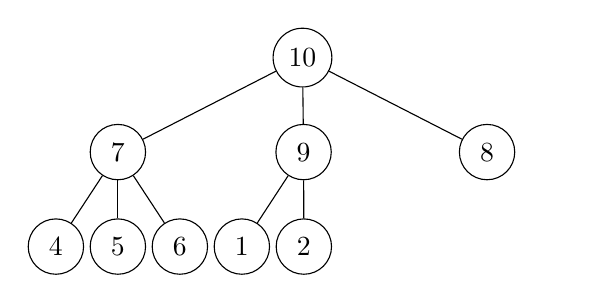
\begin{tikzpicture}
	\Tree
	[.10
		[.7
			\edge[]; [.4
			]
			\edge[]; [.5
			]
			\edge[]; [.6
			]
		]
		[.9
			\edge[]; [.1 
			]
			\edge[]; [.2 
			]
			\edge[blank]; \node[blank]{};
		]
		[.8
			\edge[blank]; \node[blank]{};
			\edge[blank]; \node[blank]{};
			\edge[blank]; \node[blank]{};
		]
	]
	\end{tikzpicture}
\end{minipage}%

~\\

\begin{parts}
  \part[4] If you are given the node with index $i$, what is the index of its parent and its $j$th child ($1 \leq j \leq k$)?

\textbf{Notice: }We assume the root is kept in $A[1]$. For your final answer, please represent it in terms of $k$, $i$ and $j$. Please use flooring or ceiling to ensure that your final answer is as tight as possible if you need, i.e. $\lfloor m \rfloor$, $\lceil m \rceil$.

    \begin{solution}
    %%%%%%%%%%%%%%%%%%%%%%%%%%%%%%%%%%%%%%%%%%%%%%%%%
    % Replace `\vspace{2in}' with your answer.
    %\vspace{2in}
    \\parent: \ $\lfloor \frac{i+k-2}{k} \rfloor$\\
	j\_th child: $k\cdot(i-1)+j+1$
	%%%%%%%%%%%%%%%%%%%%%%%%%%%%%%%%%%%%%%%%%%%%%%%%%
  \end{solution}
 
\newpage

  \part[4] What is the height of a $k$-ary heap of $n$ elements? Please show your steps.

\textbf{Notice: }For your final answer, please represent it in terms of $i$ and $n$. Please use flooring or ceiling to ensure that your final answer is as tight as possible if you need, i.e. $\lfloor m \rfloor$, $\lceil m \rceil$.

    \begin{solution}
    %%%%%%%%%%%%%%%%%%%%%%%%%%%%%%%%%%%%%%%%%%%%%%%%%
    % Replace `\vspace{2in}' with your answer.
	%\vspace{2.5in}
    \\suppose that the $k$-ary heap with $n$ elements has the height $h$\\
	it is meaningless when $k \leq 1$, so we just let $k \geq 2$\\
	and the heap is a complete $k$-ary tree, so the number of its node is 
	more than a perfect $k$-ary tree with height $h-1$, and is less than or equal
	to a perfect $k$-ary tree with height $h$\\
	and since a perfect $k$-ary tree with height $h$ has the number of node:\\
	$1+k+k^2+\cdots+k^h=\frac{k^{h+1}-1}{k-1}$\\
	so $\frac{k^{(h-1)+1}-1}{k-1} < n \leq \frac{k^{h+1}-1}{k-1}$\\
	since $k\geq 2$, so $k-1>0$, so simplify it we have\\
	$log_k{(n(k-1)+1)}-1\leq h < log_k{(n(k-1)+1)}$\\
	so we can take $h=\lceil log_k{(n(k-1)+1)}\rceil$\\
	above all, the height of heap is $\lceil log_k{(n(k-1)+1)}-1\rceil$
	%%%%%%%%%%%%%%%%%%%%%%%%%%%%%%%%%%%%%%%%%%%%%%%%%
  \end{solution}
  
  \part[4] Now we want to study the complexity of operations on $k$-ary heap. Suppose the $Push$, $Pop$ and $Heap-sort$ operations execute the same as what we mentioned in our lectures. Denote the height of the heap as $h$, please analyse the worst-case time complexity of $Push$ and $Pop$ operations on $k$-ary heap in terms of $n,h,k$ with tight bound. For heap-sort, given a built heap, explain why the worst-case number of comparisons is $\Theta(nhk)$.

    \begin{solution}
    %%%%%%%%%%%%%%%%%%%%%%%%%%%%%%%%%%%%%%%%%%%%%%%%%
    % Replace `\vspace{2in}' with your answer.
    %\vspace{2.5in}
    \\let the heap be the min heap.\\
	$push$ operation: after putting a new node into the heap, the new node need to compare with its father,
	and if its value is less than its father's, then swap the two nodes.
	for the worst case, the new node become the root of the heap, with needs to compare $n$ times,\\
	so the complexity of $push$ is $\Theta(h)$\\
	\\
	$pop$ operation: after removing the root of the heap, we put the last node to the root, and it need to compare with all its $k$ children,
	if there exist some children with less value, then we need to swap the child with minimum value with it.
	since the node have $k$ children, so we need to compare $k$ times each time. And for the worst case, the node 
	become the leaf node, so we need to repeat $h$ times above.\\
	so the complexity of $pop$ operation is $\Theta(k\cdot h)$\\
	\\
	for $heap-sort$: for the worst case, each time when we want to pop,
	the pop operation takes the worst time, and the heap-sort of $n$ elements
	requires total $n$ pop operations, so it takes time of $n\cdot$ pop()'s complexity
	=$n\cdot(k\cdot h)=nhk$\\
	so above all, the worst case of heap-sort's complexity is $\Theta(nhk)$.
	%%%%%%%%%%%%%%%%%%%%%%%%%%%%%%%%%%%%%%%%%%%%%%%%%
  \end{solution}
 

\end{parts}


\end{questions}

\end{document}